\begin{thm}{213}{\hosi 6}{京大OP 添削用問題}
 直角三角形の周の長さを$L$、内接円の半径を$r$とおく。$\dfrac{L}{r}$の最小値を求めよ。
\end{thm}

直角三角形の斜辺を$a$、1つの鋭角を$\theta$ (ただし$0<\theta<\dfrac{\pi}{2}$) とおく。
\begin{figure}[H]
 \centering
 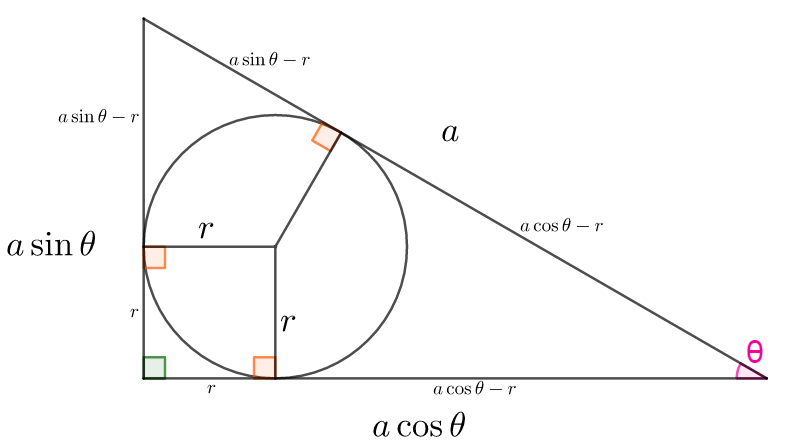
\includegraphics[width=0.6\linewidth]{../problems/Q_213/A_213.png}
\end{figure}
すると
\[ L=a(1+\cos\theta+\sin\theta) \]
である。直角三角形の面積を考えて、
\[ \frac{1}{2}Lr=\frac{1}{2}a^2\sin\theta\cos\theta \quad\dou\quad \frac{L}{r}=\frac{a^2}{r^2}\sin\theta\cos\theta \]
が成り立つ。一方で、
\[ a=(a\sin\theta-r)+(a\cos\theta-r) \quad\dou\quad \frac{a}{r}=\frac{2}{\sin\theta+\cos\theta-1} \]
である。以上のことから、
\[ \frac{L}{r}=\left(\frac{a}{r}\right)^2\sin\theta\cos\theta=\frac{4\sin\theta\cos\theta}{(\sin\theta+\cos\theta-1)^2} \]
と書ける。$t=\sin\theta+\cos\theta$とおくと、
\begin{align*}
 \frac{L}{r}&=\frac{2(t^2-1)}{(t-1)^2}=\frac{2(t+1)}{(t-1)}=2+\frac{4}{t-1}
\end{align*}
であるから、$t$を最大化すればこの値は最小となる。$t=\sqrt{2}\sin\left(\theta+\dfrac{\pi}{4}\right)$なので、$\theta=\dfrac{\pi}{4}$のときに$t$は最大値$\sqrt{2}$をとる。このとき最小値は、
\[ 2+\frac{4}{\sqrt{2}-1}=4\sqrt{2}+6 \]